\documentclass[aspectratio=169,12pt,t]{beamer}

% --- Theme: Metropolis (modern, clean) ---
\usetheme[progressbar=frametitle,numbering=fraction,block=fill]{metropolis}

% --- Fira Sans font (install texlive-fonts-extra if missing) ---
\IfFileExists{FiraSans.sty}{\usepackage[sfdefault]{FiraSans}}{}

% --- Light background with warm accent ---
\definecolor{mDarkTeal}{RGB}{35,55,59}
\definecolor{mLightBrown}{RGB}{235,228,216}
\definecolor{mAccent}{RGB}{140,70,20}

\setbeamercolor{normal text}{fg=mDarkTeal,bg=white}
\setbeamercolor{alerted text}{fg=mAccent}
\setbeamercolor{frametitle}{bg=mDarkTeal,fg=white}
\setbeamercolor{progress bar}{fg=mAccent,bg=mLightBrown}
\setbeamercolor{title separator}{fg=mAccent}
\setbeamercolor{progress bar in head/foot}{fg=mAccent,bg=mLightBrown}
\setbeamercolor{progress bar in section page}{fg=mAccent,bg=mLightBrown}

% --- Packages ---
\usepackage[utf8]{inputenc}
\usepackage{amsmath,amssymb,amsthm}
\usepackage{mathrsfs}
\usepackage{tikz}
\usetikzlibrary{arrows.meta,positioning,calc,decorations.pathreplacing,shapes,patterns}
\usepackage{pgfplots}
\pgfplotsset{compat=1.18}

% --- Semi-transparent white highlight for text on top of background images ---
\usepackage[most]{tcolorbox}

% Inline highlight: \hl{short text}
\newtcbox{\hl}{%
  nobeforeafter, tcbox raise base,
  colback=white, opacityback=0.6,
  colframe=white, opacityframe=0,
  sharp corners, boxsep=2pt, left=3pt, right=3pt, top=2pt, bottom=2pt%
}

% Block highlight: \begin{hlbox} ... \end{hlbox}  (multi-line, paragraphs, itemize)
\newtcolorbox{hlbox}[1][]{%
  enhanced, breakable,
  colback=white, opacityback=0.6,
  colframe=white, opacityframe=0,
  boxsep=3pt, left=6pt, right=6pt, top=4pt, bottom=4pt,
  sharp corners,
  {#1}%
}

% --- Custom colors for content types ---
\definecolor{defcolor}{RGB}{25,85,120}
\definecolor{thmcolor}{RGB}{140,35,35}
\definecolor{proofcolor}{RGB}{35,100,50}
\definecolor{excolor}{RGB}{140,75,10}
\definecolor{remcolor}{RGB}{90,90,90}

% --- Beamer blocks for mathematical content types (semi-transparent) ---
\tcbset{hlblockbase/.style={
  enhanced, breakable,
  coltitle=white, fonttitle=\bfseries,
  opacitybacktitle=0.8, opacityback=0.6,
  opacityframe=0,
  sharp corners,
  boxsep=1pt, left=5pt, right=5pt, top=2pt, bottom=2pt,
  toptitle=1pt, bottomtitle=1pt
}}

\newtcolorbox{defblock}[1]{hlblockbase, title={#1},
  colbacktitle=defcolor, colback=defcolor!15, colframe=defcolor}
\newtcolorbox{thmblock}[1]{hlblockbase, title={#1},
  colbacktitle=thmcolor, colback=thmcolor!15, colframe=thmcolor}
\newtcolorbox{proofblock}[1]{hlblockbase, title={#1},
  colbacktitle=proofcolor, colback=proofcolor!15, colframe=proofcolor}
\newtcolorbox{exblock}[1]{hlblockbase, title={#1},
  colbacktitle=excolor, colback=excolor!15, colframe=excolor}
\newtcolorbox{remblock}[1]{hlblockbase, title={#1},
  colbacktitle=remcolor, colback=remcolor!15, colframe=remcolor}

% --- Metadata ---
\title{Chapter 3: Numerical Sequences and Series}
\subtitle{Section: Absolute Convergence}
\author{Based on Walter Rudin's \emph{Principles of Mathematical Analysis}}
\date{}

\begin{document}

% =============================================================================
% TITLE AND OUTLINE
% =============================================================================
{
\usebackgroundtemplate{%
  
\includegraphics[width=\paperwidth,height=\paperheight,keepaspectratio=false]{chapter_03_bg_00.png}%
}
\begin{frame}[plain]
  \titlepage
  \note{
    Welcome back to Chapter 3 of Principles of Mathematical Analysis. In
    this short but important section we introduce the idea of absolute
    convergence. A series converges absolutely when the series of absolute
    values converges. The central fact is that absolute convergence is a
    stronger condition: if a series converges absolutely, then it converges
    in the ordinary sense as well. We will prove this in a single clean
    step, and then step back to see why absolute convergence is the
    dividing line that organizes everything we have done with series so
    far. The convergence tests we built earlier, the comparison test and
    the root and ratio tests, all turn out to be tests for absolute
    convergence. Let's begin.
  }
\end{frame}
}

{
\usebackgroundtemplate{%
  
\includegraphics[width=\paperwidth,height=\paperheight,keepaspectratio=false]{chapter_03_bg_01.png}%
}
\begin{frame}[c]{Outline}
  \begin{center}
    \tableofcontents
  \end{center}
  \note{
    Here is the plan. We start with motivation, recalling the difference
    between a series and the series of its absolute values, and asking why
    that distinction matters. Then we give the definition of absolute
    convergence. Next we state and prove Theorem 3.45, the result that
    absolute convergence implies convergence. After that we work through
    the remarks in 3.46, which explain how absolute convergence relates to
    our convergence tests, what nonabsolute convergence means, and why
    absolutely convergent series behave so nicely. Finally we summarize.
  }
\end{frame}

% =============================================================================
\section{Motivation}
% =============================================================================

% --- Build 1/3 ---
\begin{frame}{Why Absolute Convergence?}
  \begin{hlbox}
  \begin{itemize}
    \item Given $\Sigma a_n$, also look at the series of \alert{sizes} $\Sigma |a_n|$
  \end{itemize}
  \end{hlbox}

  \note{
    Let's set the stage. So far we have studied a series sum of "a" sub
    "n", asking whether its partial sums settle down to a limit. But there
    is a second series hiding in plain sight: the series of absolute
    values, sum of the size of "a" sub "n". This second series throws away
    all the sign and cancellation information and just asks how big the
    terms are. The relationship between these two series is the whole
    subject of this section. Next, let's see why the two can behave very
    differently.
  }
\end{frame}

% --- Build 2/3 ---
\begin{frame}{Why Absolute Convergence?}
  \begin{hlbox}
  \begin{itemize}
    \item Given $\Sigma a_n$, also look at the series of \alert{sizes} $\Sigma |a_n|$
    \item Cancellation can save a series:\\
      $\sum \frac{(-1)^n}{n}$
      converges, but $\sum \frac{1}{n}$ \alert{diverges}
  \end{itemize}
  \end{hlbox}

  \note{
    Here is the key tension, shown on the slide. The alternating harmonic
    series, sum of negative one to the "n" over "n", converges. We proved
    this back in the section on summation by parts, using the alternating
    series test. Yet if we replace every term by its absolute value we get
    the ordinary harmonic series, sum of one over "n", which diverges.
    So this series only converges because of cancellation between positive
    and negative terms. Its convergence is fragile. Next, let's name the
    stronger, more robust kind of convergence.
  }
\end{frame}

% --- Build 3/3 ---
\begin{frame}{Why Absolute Convergence?}
  \begin{hlbox}
  \begin{itemize}
    \item Given $\Sigma a_n$, also look at the series of \alert{sizes} $\Sigma |a_n|$
    \item Cancellation can save a series:\\
      $\sum \frac{(-1)^n}{n}$
      converges, but $\sum \frac{1}{n}$ \alert{diverges}
    \item \textbf{Question:} when does convergence \alert{not} rely on cancellation?
  \end{itemize}
  \end{hlbox}

  \note{
    This leads to the central question of the section, stated in the third
    bullet. When does a series converge for a more robust reason, one that
    does not depend on delicate cancellation between terms? The answer is
    absolute convergence: when the series of sizes already converges, the
    original series is convergent in the strongest possible sense, and as
    we will see it behaves almost like a finite sum. Let's make this
    precise with a definition.
  }
\end{frame}

}

{
\usebackgroundtemplate{%
  
\includegraphics[width=\paperwidth,height=\paperheight,keepaspectratio=false]{chapter_03_bg_02.png}%
}
% =============================================================================
\section{Definition}
% =============================================================================

\begin{frame}{Absolute Convergence}
  \begin{defblock}{Definition: Absolute Convergence}
    The series $\Sigma a_n$ is said to \alert{converge absolutely} if the
    series $\Sigma |a_n|$ converges.
  \end{defblock}

  \vspace{0.8em}
  \begin{hlbox}
  \textbf{Note:} the terms $a_n$ may be \emph{real or complex}; $|a_n|$ is the
  absolute value (or modulus).
  \end{hlbox}

  \note{
    Here is the definition, shown in the blue box. We say the series sum of
    "a" sub "n" converges absolutely when the series of absolute values,
    sum of the size of "a" sub "n", converges. Notice this is a statement
    about a different series, the one built from the sizes of the terms.
    The terms themselves can be real numbers or complex numbers; in either
    case the size is the absolute value, or for complex numbers the
    modulus. Because the sizes are nonnegative real numbers, we can attack
    the series of sizes with all the tools we developed for series of
    nonnegative terms. Next, the main theorem.
  }
\end{frame}

}

{
\usebackgroundtemplate{%
  
\includegraphics[width=\paperwidth,height=\paperheight,keepaspectratio=false]{chapter_03_bg_03.png}%
}
% =============================================================================
\section{Main Result}
% =============================================================================

\begin{frame}{Theorem 3.45}
  \begin{thmblock}{Theorem 3.45}
    If $\Sigma a_n$ converges \alert{absolutely}, then $\Sigma a_n$
    \alert{converges}.
  \end{thmblock}

  \vspace{0.8em}
  \begin{center}
  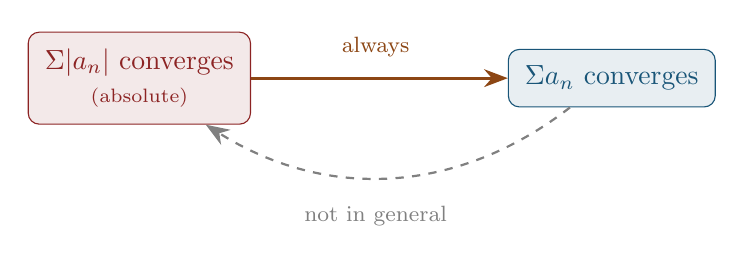
\begin{tikzpicture}[scale=1.0]
    \node[draw, thmcolor, rounded corners, fill=thmcolor!10, align=center,
          inner sep=6pt] (abs) at (0,0) {$\Sigma|a_n|$ converges\\ \scriptsize(absolute)};
    \node[draw, defcolor, rounded corners, fill=defcolor!10, align=center,
          inner sep=6pt] (con) at (6,0) {$\Sigma a_n$ converges};
    \draw[-{Stealth[length=3mm]}, very thick, mAccent] (abs) -- (con);
    \node[mAccent, above] at (3,0.15) {\footnotesize always};
    \draw[-{Stealth[length=3mm]}, thick, gray, dashed] (con) to[bend left=35] (abs);
    \node[gray, below] at (3,-1.5) {\footnotesize not in general};
  \end{tikzpicture}
  \end{center}

  \note{
    Here is the main result, Theorem 3.45. If a series converges
    absolutely, then it converges. In words, the stronger condition on the
    series of sizes guarantees ordinary convergence of the original series.
    The diagram captures the logic. The solid orange arrow on top points
    from absolute convergence to convergence, because that implication
    always holds. The faint dashed arrow curving back the other way is
    labeled not in general, because the reverse fails: the alternating
    harmonic series converges without converging absolutely. So absolute
    convergence is the genuinely stronger condition. Let's prove the solid
    arrow.
  }
\end{frame}

}

{
\usebackgroundtemplate{%
  
\includegraphics[width=\paperwidth,height=\paperheight,keepaspectratio=false]{chapter_03_bg_04.png}%
}
% =============================================================================
\section{Proof}
% =============================================================================

\begin{frame}{Proof Strategy: Theorem 3.45}
  \begin{hlbox}
  \textbf{Goal:} from convergence of $\Sigma|a_n|$, deduce convergence of $\Sigma a_n$.

  \vspace{1em}
  \textbf{Tools:}
  \begin{enumerate}
    \item The \alert{triangle inequality} for finite sums.
    \item The \alert{Cauchy criterion} for series (Theorem 3.22).
  \end{enumerate}
  \end{hlbox}

  \note{
    Before the formal proof, here is the strategy. Our goal is to start
    from the assumption that the series of sizes converges, and conclude
    that the original series converges. We will use just two tools. First,
    the triangle inequality, which bounds the size of a finite sum by the
    sum of the sizes. Second, the Cauchy criterion for series, Theorem
    3.22, which lets us prove convergence without knowing the limit in
    advance. The idea is to transfer the Cauchy condition from the series
    of sizes, where we are given it, over to the original series, where we
    want it. Let's recall the Cauchy criterion.
  }
\end{frame}

\begin{frame}{Proof --- Step 1: Recall the Cauchy Criterion}
  \begin{thmblock}{Recall: Theorem 3.22 (Cauchy Criterion)}
    $\Sigma a_n$ converges if and only if for every $\varepsilon > 0$ there is
    an integer $N$ such that
    \[
      \left| \sum_{k=n}^{m} a_k \right| \leq \varepsilon
      \qquad (m \geq n \geq N).
    \]
  \end{thmblock}

  \note{
    Let's recall the tool, shown in the red box. The Cauchy criterion,
    Theorem 3.22, says a series converges exactly when its tail sums can be
    made arbitrarily small. Precisely, for every epsilon greater than zero
    there is an integer capital "N" so that the size of any block of terms
    from index "n" to index "m" stays below epsilon, as long as both
    indices are at least capital "N". The advantage is that this is an
    internal test: it never mentions the limit, only the terms. Since we
    are assuming the series of sizes converges, that series satisfies this
    same criterion. Next, we use the triangle inequality to connect the
    two.
  }
\end{frame}

\begin{frame}{Proof --- Step 2: The Key Inequality}
  \begin{proofblock}{Triangle inequality for finite sums}
    \[
      \left| \sum_{k=n}^{m} a_k \right| \;\leq\; \sum_{k=n}^{m} |a_k|.
    \]
  \end{proofblock}

  \vspace{0.6em}
  \begin{hlbox}
  The size of a block of $\Sigma a_n$ is controlled by the corresponding
  block of $\Sigma |a_n|$.
  \end{hlbox}

  \note{
    Here is the heart of the proof, the inequality in the green box. For
    any finite block of terms, the size of the sum is at most the sum of
    the sizes. This is just the familiar triangle inequality, the size of
    "x" plus "y" is at most the size of "x" plus the size of "y", extended
    from two terms to a whole block by applying it over and over. Its
    importance is that it links the two series term by term: whatever a
    block of the original series does, it is trapped underneath the same
    block of the series of sizes. So if we can make the blocks of the
    series of sizes small, the blocks of the original series are forced to
    be small too. Next, we combine the two facts.
  }
\end{frame}

\begin{frame}{Proof --- Step 3: Combine and Conclude}
  \begin{hlbox}
  Given $\varepsilon > 0$, apply the Cauchy criterion to $\Sigma|a_n|$:
  there is $N$ with
  \[
    \sum_{k=n}^{m} |a_k| \leq \varepsilon \qquad (m \geq n \geq N).
  \]
  Then, by Step 2,
  \[
    \left| \sum_{k=n}^{m} a_k \right| \;\leq\; \sum_{k=n}^{m} |a_k|
    \;\leq\; \varepsilon \qquad (m \geq n \geq N).
  \]
  So $\Sigma a_n$ satisfies the Cauchy criterion. \alert{Hence it converges.}
  \end{hlbox}

  \note{
    Now we put the pieces together. Fix any epsilon greater than zero.
    Because the series of sizes converges, the Cauchy criterion gives an
    integer capital "N" beyond which every block of sizes is at most
    epsilon. Now chain the inequalities, as on the slide: the size of a
    block of the original series is at most the block of sizes, which is at
    most epsilon. So the original series also satisfies the Cauchy
    criterion, with the very same capital "N". By Theorem 3.22 the original
    series converges. That completes the proof, and the boxed statement
    records the result. Next, some remarks that put this theorem in
    context.
  }
\end{frame}

}

{
\usebackgroundtemplate{%
  
\includegraphics[width=\paperwidth,height=\paperheight,keepaspectratio=false]{chapter_03_bg_05.png}%
}
% =============================================================================
\section{Remarks and Consequences}
% =============================================================================

\begin{frame}{Remark 3.46 --- Positive Terms}
  \begin{remblock}{Remark 3.46 (i)}
    For series of \alert{nonnegative} terms, absolute convergence is the
    \alert{same} as convergence.
  \end{remblock}

  \vspace{0.6em}
  \begin{hlbox}
  If $a_n \geq 0$, then $|a_n| = a_n$, so $\Sigma a_n$ and $\Sigma|a_n|$ are
  the \emph{same series}.
  \end{hlbox}

  \note{
    The first remark is a simple but useful observation, in the gray box.
    For a series whose terms are all nonnegative, absolute convergence and
    ordinary convergence are exactly the same thing. The reason, on the
    slide, is immediate: if every term "a" sub "n" is nonnegative, then its
    absolute value equals the term itself, so the series of sizes is
    literally the same series. This is why all the work we did on series of
    nonnegative terms transfers directly to absolute convergence. Next, the
    case where the two notions truly differ.
  }
\end{frame}

\begin{frame}{Remark 3.46 --- Nonabsolute Convergence}
  \begin{remblock}{Definition (nonabsolute convergence)}
    If $\Sigma a_n$ converges but $\Sigma|a_n|$ \alert{diverges}, we say
    $\Sigma a_n$ converges \alert{nonabsolutely}.
  \end{remblock}

  \vspace{0.6em}
  \begin{hlbox}
  Example: $\displaystyle \sum \frac{(-1)^n}{n}$ converges nonabsolutely
  (Theorem 3.43).
  \end{hlbox}

  \note{
    The second remark introduces a name for the fragile case. If a series
    converges, yet the series of its sizes diverges, we say the series
    converges nonabsolutely. The example, shown on the slide, is our old
    friend the alternating harmonic series. It converges by the alternating
    series test, Theorem 3.43, but the harmonic series of its absolute
    values diverges. So nonabsolute convergence is exactly the phenomenon
    we flagged in the motivation: convergence that depends entirely on
    cancellation. Next, how this connects to our convergence tests.
  }
\end{frame}

% --- Build 1/2 ---
\begin{frame}{Remark 3.46 --- Our Tests Are Absolute Tests}
  \begin{hlbox}
  \begin{itemize}
    \item The \alert{comparison}, \alert{root}, and \alert{ratio} tests all test
      for \alert{absolute} convergence.
  \end{itemize}
  \end{hlbox}

  \note{
    The third remark is a clarifying one. Look back at the convergence
    tests we have built: the comparison test, the root test, and the ratio
    test. Each of them works by bounding the sizes of the terms. So in
    truth they are all tests for absolute convergence. When one of them
    succeeds, it proves the stronger statement that the series of sizes
    converges. The flip side is on the next build: they say nothing about
    nonabsolute convergence.
  }
\end{frame}

% --- Build 2/2 ---
\begin{frame}{Remark 3.46 --- Our Tests Are Absolute Tests}
  \begin{hlbox}
  \begin{itemize}
    \item The \alert{comparison}, \alert{root}, and \alert{ratio} tests all test
      for \alert{absolute} convergence.
    \item They give \alert{no} information about nonabsolutely convergent series.
    \item \textbf{Summation by parts} can sometimes handle those instead.
  \end{itemize}
  \end{hlbox}

  \note{
    Continuing the third remark: because those tests detect only absolute
    convergence, they cannot tell us anything about a nonabsolutely
    convergent series. For a series like the alternating harmonic series,
    the root and ratio tests are silent. The right tool there is summation
    by parts, from the previous section, which gave us Dirichlet's test and
    the alternating series test. So the two halves of our theory fit
    together: absolute-value tests on one side, summation by parts on the
    other. Next, a note on power series.
  }
\end{frame}

\begin{frame}{Remark 3.46 --- Power Series}
  \begin{remblock}{Remark 3.46 (continued)}
    A power series converges \alert{absolutely} in the \alert{interior} of its
    circle of convergence.
  \end{remblock}

  \vspace{0.6em}
  \begin{center}
  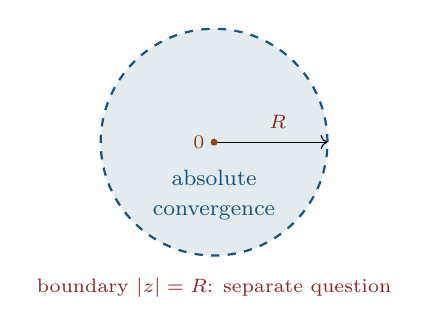
\begin{tikzpicture}[scale=0.9]
    \draw[fill=defcolor!12, draw=defcolor, thick, dashed] (0,0) circle (1.6);
    \node[defcolor] at (0,-0.5) {\footnotesize absolute};
    \node[defcolor] at (0,-1.0) {\footnotesize convergence};
    \draw[->] (0,0) -- (1.6,0);
    \node[thmcolor, above] at (0.9,0.05) {\scriptsize $R$};
    \fill[mAccent] (0,0) circle (1.4pt);
    \node[mAccent, left] at (0,0) {\scriptsize $0$};
    \node[thmcolor] at (0,-2.05) {\scriptsize boundary $|z|=R$: separate question};
  \end{tikzpicture}
  \end{center}

  \note{
    The fourth remark connects to power series. Recall from Theorem 3.39
    that a power series has a radius of convergence capital "R". The remark
    sharpens that picture: inside the circle, that is, wherever the size of
    "z" is strictly less than capital "R", the convergence is actually
    absolute. The diagram shows the disk of radius capital "R" shaded as
    the region of absolute convergence, with the center at zero. This
    follows from the root test applied to the terms. The boundary, where
    the size of "z" equals capital "R", is a separate and often delicate
    question, exactly the kind that summation by parts addresses. Next, the
    biggest payoff of absolute convergence.
  }
\end{frame}

% --- Build 1/2 ---
\begin{frame}{Remark 3.46 --- Why It Matters}
  \begin{remblock}{Absolutely convergent series behave like finite sums}
    We may \alert{rearrange} the terms and \alert{multiply} two such series
    term by term, without changing the sum.
  \end{remblock}

  \note{
    The final remark is the deepest, in the gray box. Absolutely convergent
    series behave very much like ordinary finite sums. With a finite sum we
    freely reorder the terms and multiply two sums out term by term, and
    nothing changes. The remarkable fact, which we will prove in the coming
    sections, is that absolute convergence is exactly the condition that
    lets us do the same with infinite series: we may rearrange the order of
    the terms and we may multiply two series together, all without
    affecting the sum. Next, the warning for the other case.
  }
\end{frame}

% --- Build 2/2 ---
\begin{frame}{Remark 3.46 --- Why It Matters}
  \begin{remblock}{Absolutely convergent series behave like finite sums}
    We may \alert{rearrange} the terms and \alert{multiply} two such series
    term by term, without changing the sum.
  \end{remblock}

  \vspace{0.6em}
  \begin{hlbox}
  \textbf{Warning:} for \alert{nonabsolutely} convergent series this
  \alert{fails} --- rearranging can change the sum (Theorem 3.54).
  \end{hlbox}

  \note{
    But here is the warning, on the second line. For nonabsolutely
    convergent series, all of this breaks down. Rearranging the terms can
    actually change the sum, and in fact, by a theorem of Riemann that we
    will meet as Theorem 3.54, a nonabsolutely convergent series of real
    numbers can be rearranged to converge to any value we like, or even to
    diverge. So absolute convergence is not a technicality; it is precisely
    the license that makes infinite series safe to manipulate. Let's
    summarize.
  }
\end{frame}

}

{
\usebackgroundtemplate{%
  
\includegraphics[width=\paperwidth,height=\paperheight,keepaspectratio=false]{chapter_03_bg_06.png}%
}
% =============================================================================
\section{Summary}
% =============================================================================

% --- Build 1/4 ---
\begin{frame}{Summary}
  \begin{hlbox}
  \textbf{Key takeaways from this section:}
  \begin{itemize}
    \item \alert{Definition:} $\Sigma a_n$ converges absolutely if
      $\Sigma|a_n|$ converges.
  \end{itemize}
  \end{hlbox}

  \note{
    Let's review what we covered. First, the definition: a series converges
    absolutely when the series of the absolute values of its terms
    converges. This is a condition on the sizes alone, ignoring sign and
    cancellation. Next, the main theorem.
  }
\end{frame}

% --- Build 2/4 ---
\begin{frame}{Summary}
  \begin{hlbox}
  \textbf{Key takeaways from this section:}
  \begin{itemize}
    \item \alert{Definition:} $\Sigma a_n$ converges absolutely if
      $\Sigma|a_n|$ converges.
    \item \alert{Theorem 3.45:} absolute convergence $\Rightarrow$ convergence,
      via the triangle inequality plus the Cauchy criterion.
  \end{itemize}
  \end{hlbox}

  \note{
    Second, the main result, Theorem 3.45: absolute convergence implies
    ordinary convergence. The proof was short and clean. The triangle
    inequality bounds each block of the original series by the corresponding
    block of the series of sizes, and the Cauchy criterion then transfers
    convergence from one to the other. Next, the converse.
  }
\end{frame}

% --- Build 3/4 ---
\begin{frame}{Summary}
  \begin{hlbox}
  \textbf{Key takeaways from this section:}
  \begin{itemize}
    \item \alert{Definition:} $\Sigma a_n$ converges absolutely if
      $\Sigma|a_n|$ converges.
    \item \alert{Theorem 3.45:} absolute convergence $\Rightarrow$ convergence,
      via the triangle inequality plus the Cauchy criterion.
    \item \alert{Converse fails:} $\sum (-1)^n/n$ converges nonabsolutely;
      our comparison, root, and ratio tests are absolute tests.
  \end{itemize}
  \end{hlbox}

  \note{
    Third, the converse fails. A series can converge without converging
    absolutely; the alternating harmonic series is the standard example,
    and we call this nonabsolute convergence. Our main convergence tools,
    the comparison, root, and ratio tests, are really tests for absolute
    convergence, so they say nothing about the nonabsolute case. Summation
    by parts fills that gap. Next, why we care.
  }
\end{frame}

% --- Build 4/4 ---
\begin{frame}{Summary}
  \begin{hlbox}
  \textbf{Key takeaways from this section:}
  \begin{itemize}
    \item \alert{Definition:} $\Sigma a_n$ converges absolutely if
      $\Sigma|a_n|$ converges.
    \item \alert{Theorem 3.45:} absolute convergence $\Rightarrow$ convergence,
      via the triangle inequality plus the Cauchy criterion.
    \item \alert{Converse fails:} $\sum (-1)^n/n$ converges nonabsolutely;
      our comparison, root, and ratio tests are absolute tests.
    \item \alert{Payoff:} absolutely convergent series can be rearranged and
      multiplied like finite sums.
  \end{itemize}

  \vspace{0.4em}
  \textbf{Coming up next:} addition and multiplication of series.
  \end{hlbox}

  \note{
    Finally, the payoff. Absolute convergence is exactly the condition
    that lets us treat an infinite series like a finite sum: we may
    rearrange its terms and multiply two such series together without
    changing the result, while for nonabsolutely convergent series this can
    fail dramatically. This sets up the next section, on the addition and
    multiplication of series, where we will see these manipulations carried
    out and proved. Thanks for watching, and see you in the next section.
  }
\end{frame}
}

\end{document}
